\documentclass[hyperref,UTF8,12pt,a4paper]{ctexart}
\usepackage{amsmath}
\usepackage{amsfonts}

\usepackage{geometry}
\usepackage{tikz}
\geometry{left=1in,right=1in,top=1in,bottom=1in}

%% make section title left aligned
\ctexset{section/format=\Large\bfseries}

%% pseudo-code
% \usepackage{algorithm}
% \usepackage{algpseudocode}

%% minted
\usepackage{minted}

%% plots
% \usepackage{pgfplots}
% \pgfplotsset{compat = newest}

\hypersetup{
	colorlinks=true,
	linkcolor=black
}

\usepackage{titling}
\pretitle{\begin{center}\fontsize{30pt}{30pt}\selectfont}
\posttitle{\end{center}}

\usepackage{ulem}

\title{关注永雏塔菲喵}
\author{永雏塔菲}
\date{\today}

\begin{document}
\maketitle
\newpage

\section{题目}

掌握 openGauss 数据库镜像安装部署方法(或掌握 openGauss 数据库安装部署方法); 

熟悉并掌握 openGauss 数据库的基本操作。

\section{源程序清单和结果}

\begin{enumerate}
\item 建立用户 tom,创建数据库 ST,使得 tom 拥有数据库 ST % 1

\begin{minted}{sql}
create user tom with password 'Passw0rd';
create database st owner tom;
\end{minted}

\item 以 tom 用户连接数据库 ST % 2

\begin{minted}{bash}
gsql -d st -U tom -P Passw0rd -p 26000 -h localhost -r
\end{minted}

\item 创建 SCHEMA % 3

\begin{minted}{sql}
create schema tom authorization tom;
\end{minted}

\item 建立课程表

\begin{minted}{sql}
create table if not exists c (
  cno int not null,
  cname varchar(20) not null,
  cpno int,
  ccredit int not null,
  primary key (cno),
  foreign key (cpno) references c(cno),
  check (ccredit > 0)
);
\end{minted}

\begin{center}
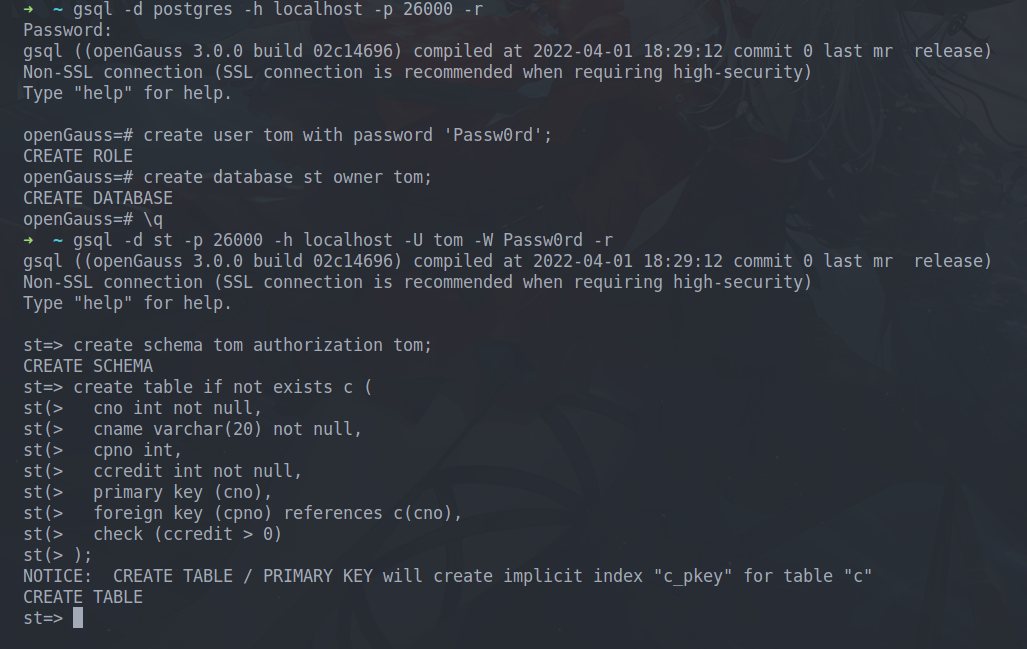
\includegraphics[width=0.8\textwidth]{1-4.png}
\end{center}

\item 建立学生表

\begin{minted}{sql}
create table if not exists s (
  sclass int not null,
  sno int not null,
  sname varchar(20) not null,
  ssex varchar(5) not null,
  sage int not null,
  sdept varchar(20) not null,
  primary key (sclass, sno),
  check (ssex = '男' or ssex = '女' or ssex = '其他'),
  check (sage > 0)
);
\end{minted}

\begin{center}
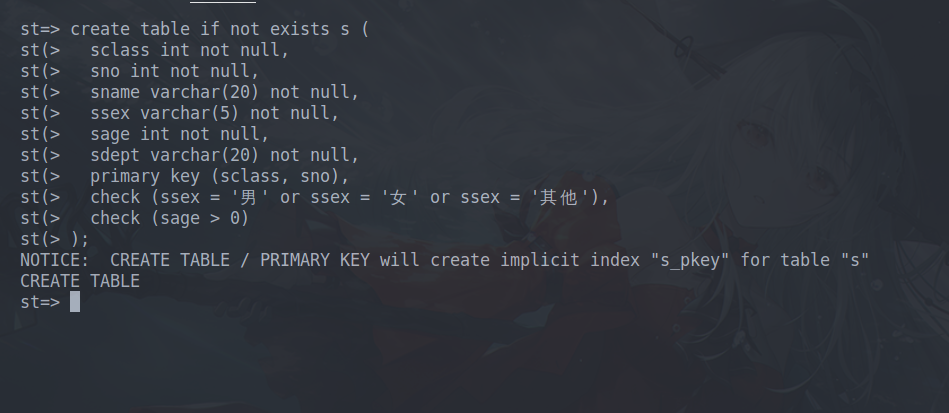
\includegraphics[width=0.8\textwidth]{5.png}
\end{center}

\item 建立选课表

\begin{minted}{sql}
create table if not exists sc (
  sclass int not null,
  sno int not null,
  cno int not null,
  grade int not null,
  primary key (sclass, sno, cno),
  foreign key (sclass, sno) references s(sclass, sno),
  foreign key (cno) references c(cno),
  check (grade >= 0)
);
\end{minted}

\begin{center}
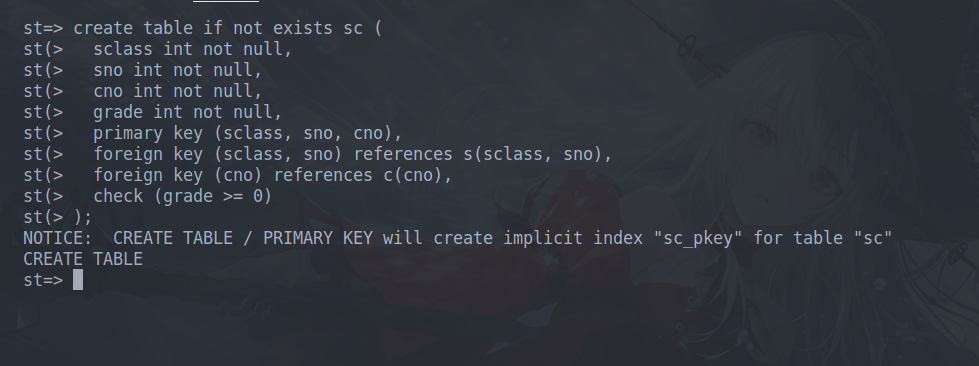
\includegraphics[width=0.8\textwidth]{6.png}
\end{center}

\item 分别向课程表、学生表、选课表中插入数据

\begin{minted}{sql}
insert into c
values
  (1, '数据库', 5, 4),
  (2, '数学', NULL, 2),
  (3, '信息系统', 1, 4),
  (4, '操作系统', 6, 3),
  (5, '数据结构', 7, 4),
  (6, '数据处理', NULL, 2),
  (7, 'PASCAL语言', 6, 4);

insert into s
values
  (1, 1, '李勇', '男', 20, 'IS'),
  (1, 2, '刘晨', '女', 19, 'IS'),
  (1, 3, '刘朋', '男', 20, 'IS'),
  (2, 1, '王敏', '女', 18, 'MA'),
  (2, 2, '张锋', '男', 19, 'MA'),
  (2, 3, '李敏', '男', 20, 'MA');

insert into sc
values
  (1, 1, 1, 92),
  (1, 1, 2, 85),
  (1, 1, 3, 88),
  (1, 2, 2, 90),
  (1, 2, 3, 80),
  (2, 1, 1, 75),
  (2, 1, 2, 92),
  (2, 2, 2, 87),
  (2, 2, 3, 89),
  (2, 3, 1, 90);
\end{minted}

\begin{center}
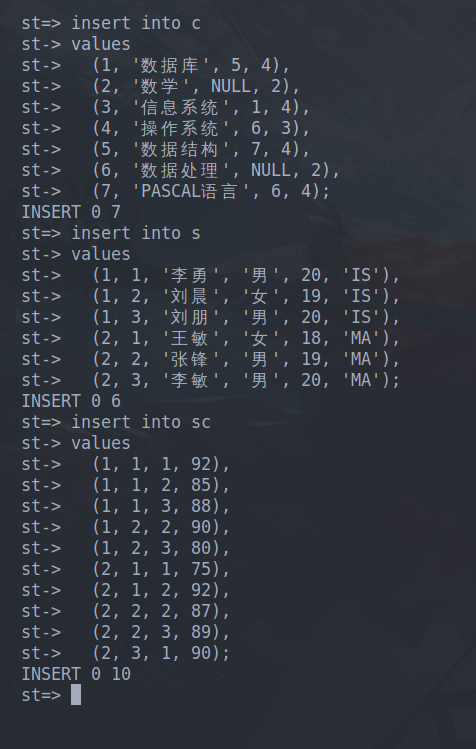
\includegraphics[width=0.8\textwidth]{7.png}
\end{center}

\item 查询所有学生的详细信息(包含学生、选课及课程信息) 

\begin{minted}{sql}
select s.sclass, s.sno, sname, ssex, sage, sdept, cname, grade
from s, sc, c
where s.sclass = sc.sclass
  and s.sno = sc.sno
  and sc.cno = c.cno;
\end{minted}

\begin{center}
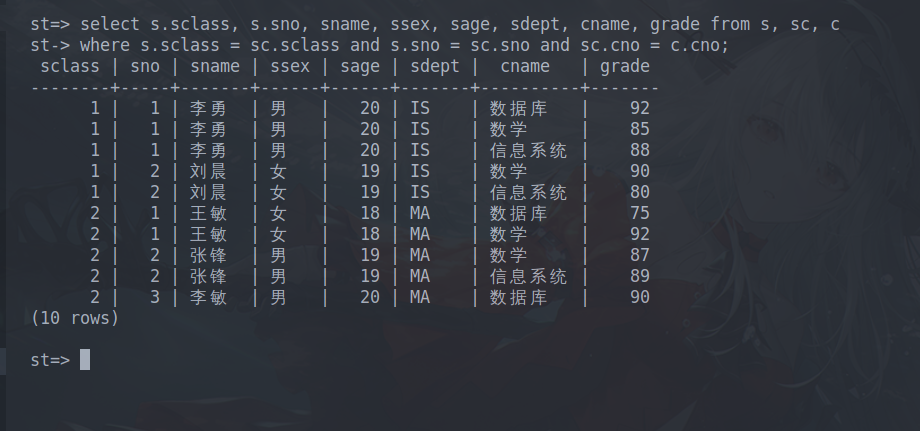
\includegraphics[width=0.8\textwidth]{8.png}
\end{center}

\item 查询 1 班的学生学号及姓名

\begin{minted}{sql}
select sno, sname
from s
where sclass = 1;
\end{minted}

\begin{center}
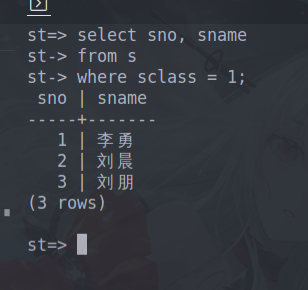
\includegraphics[width=0.8\textwidth]{9.png}
\end{center}

\item 查询‘刘晨’的出生年

\begin{minted}{sql}
select 2022 - sage as birth_year
from s
where sname = '刘晨';
\end{minted}

\begin{center}
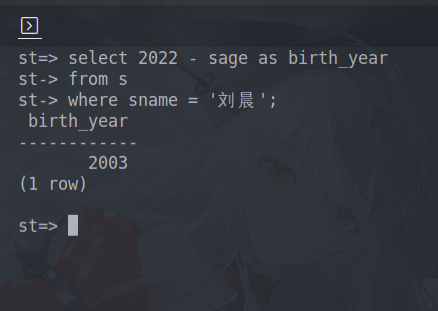
\includegraphics[width=0.8\textwidth]{10.png}
\end{center}

\item 查询姓‘刘’的学生的详细情况(包括学生表、选课表及课程表的全部信息)

\begin{minted}{sql}
select s.sclass, s.sno, sname, ssex, sage, sdept, cname, grade
from s, sc, c
where s.sclass = sc.sclass
  and s.sno = sc.sno
  and sc.cno = c.cno
  and sname like '刘%';
\end{minted}

\begin{center}
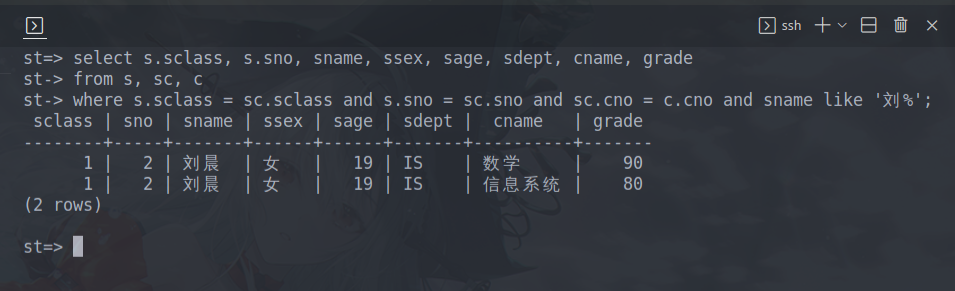
\includegraphics[width=0.8\textwidth]{11.png}
\end{center}

\item 查询选修了 1 号课的学生姓名、性别、成绩

\begin{minted}{sql}
select sname, ssex, grade
from s, sc
where s.sclass = sc.sclass
  and s.sno = sc.sno
  and sc.cno = 1;
\end{minted}

\begin{center}
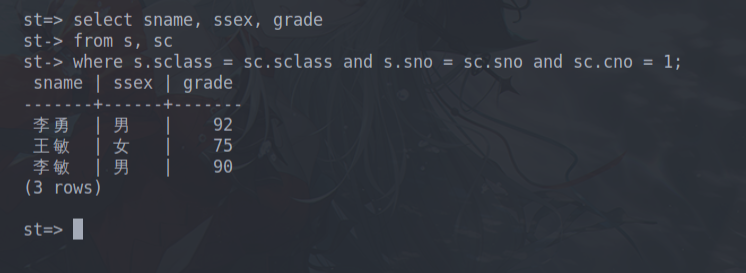
\includegraphics[width=0.8\textwidth]{12.png}
\end{center}

\item 查询没有先行课课程的课程号和课程名

\begin{minted}{sql}
select cno, cname
from c
where cpno is null;
\end{minted}

\begin{center}
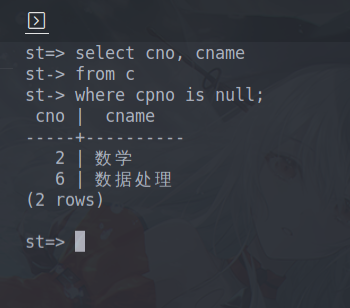
\includegraphics[width=0.8\textwidth]{13.png}
\end{center}

\item 查询 2 班的所有女生的情况

\begin{minted}{sql}
select s.sclass, s.sno, sname, ssex, sage, sdept, cname, grade
from s, sc, c
where s.sclass = sc.sclass
  and s.sno = sc.sno
  and sc.cno = c.cno
  and ssex = '女'
  and s.sclass = 2;
\end{minted}

\begin{center}
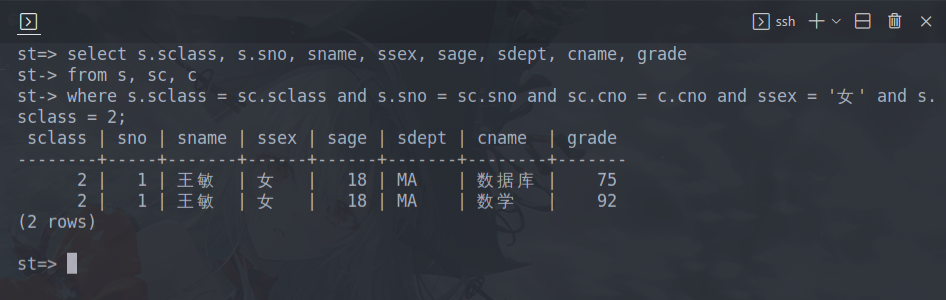
\includegraphics[width=0.8\textwidth]{14.png}
\end{center}

\item 查询学分为 2 到 3 之间的课程号及课程名

\begin{minted}{sql}
select cno, cname
from c
where ccredit >= 2
  and ccredit <= 3;
\end{minted}

\begin{center}
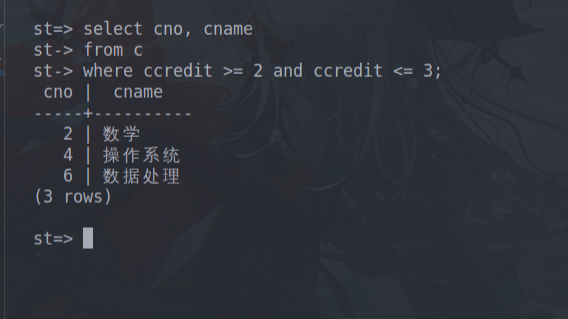
\includegraphics[width=0.8\textwidth]{15.png}
\end{center}

\item 查询选修 1 号课的学生的班号、学号、姓名、课程名及成绩,要求成绩按照递减排序输出

\begin{minted}{sql}
select s.sclass, s.sno, sname, cname, grade
from s, sc, c
where s.sclass = sc.sclass
  and s.sno = sc.sno
  and sc.cno = c.cno
  and sc.cno = 1
order by grade desc;
\end{minted}

\begin{center}
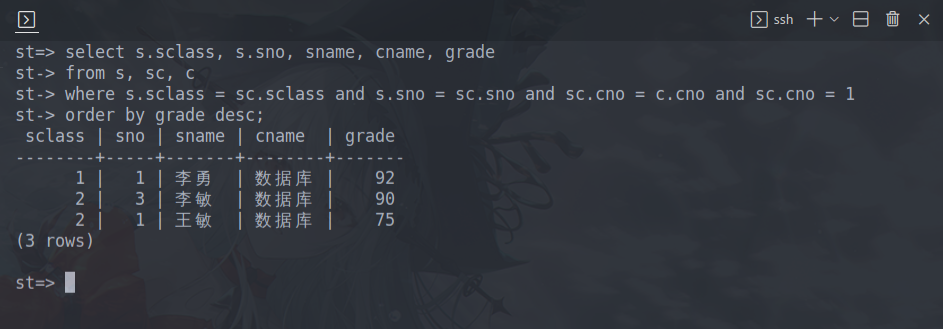
\includegraphics[width=0.8\textwidth]{16.png}
\end{center}

\item 查询 2 班至少选修一门其先行课为 1 号课的学生的班号、学号、姓名、性别、系、课程号及成绩

\begin{minted}{sql}
select s.sclass, s.sno, sname, ssex, sdept, c.cno, grade
from s, sc, c
where s.sclass = sc.sclass
  and s.sno = sc.sno
  and sc.cno = c.cno
  and c.cpno = 1
  and s.sclass = 2;
\end{minted}

\begin{center}
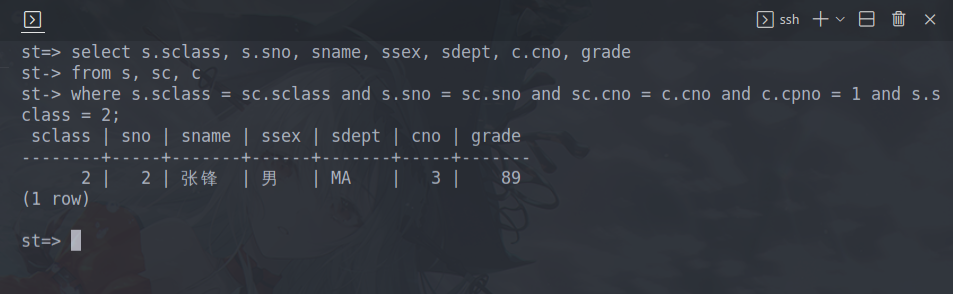
\includegraphics[width=0.8\textwidth]{17.png}
\end{center}

\item 查询 2 号科成绩最高的学生班号、学号、姓名

\begin{minted}{sql}
select s.sclass, s.sno, sname
from s, sc
where s.sclass = sc.sclass
  and s.sno = sc.sno
  and sc.cno = 2
order by grade desc limit 1;

\end{minted}

\begin{center}
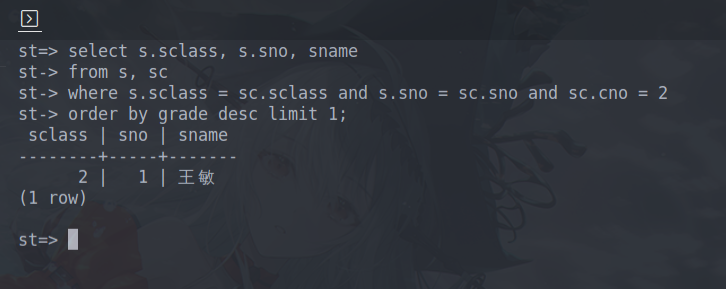
\includegraphics[width=0.8\textwidth]{18.png}
\end{center}

\item 查询 1 班 2 号课成绩最低的学生班号、学号 

\begin{minted}{sql}
select sclass, sno
from sc
where sclass = 1
  and cno = 2
order by grade asc limit 1;
\end{minted}

\begin{center}
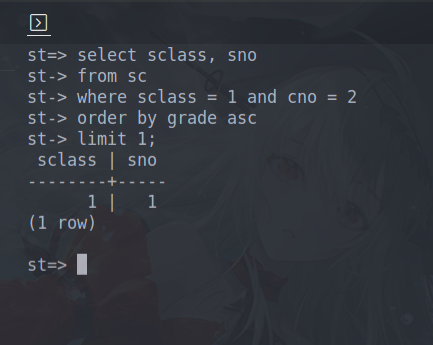
\includegraphics[width=0.8\textwidth]{19.png}
\end{center}

\item 查询选修 2 号课且成绩不是最低的同学班号、学号

\begin{minted}{sql}
select sclass, sno
from sc
where cno = 2
  and grade > any (
    select grade
    from sc
    where cno = 2
  );
\end{minted}

\begin{center}
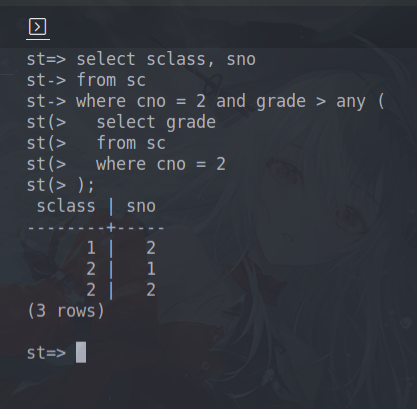
\includegraphics[width=0.8\textwidth]{20.png}
\end{center}

\item 查询包含 2 班 1 号同学所选全部课程的同学的班号、学号

\begin{minted}{sql}
select sclass, sno
from s as a
where not exists (
  select *
  from sc as b
  where b.sclass = 2
    and b.sno = 1
    and b.cno not in (
      select cno
      from sc as c
      where c.sclass = a.sclass
        and c.sno = a.sno
    )
);
\end{minted}

\begin{center}
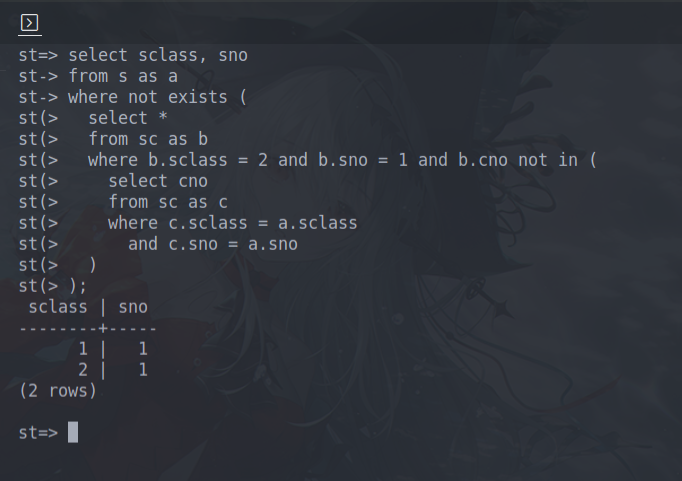
\includegraphics[width=0.8\textwidth]{21.png}
\end{center}

\item 查询选修每门课程的课程号及人数

\begin{minted}{sql}
select cno, count(*) as num
from sc
group by cno;
\end{minted}

\begin{center}
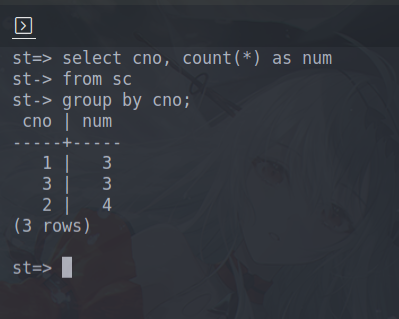
\includegraphics[width=0.8\textwidth]{22.png}
\end{center}

\item 查询选修三门课的同学班号、学号、姓名、课程名及成绩

\begin{minted}{sql}
select s.sclass, s.sno, sname, cname, grade
from s, sc, c
where s.sclass = sc.sclass
  and s.sno = sc.sno
  and c.cno = sc.cno
  and (sc.sclass, sc.sno) in (
    select sclass, sno
    from sc
    group by sclass, sno
    having count(*) = 3
  );
\end{minted}

\begin{center}
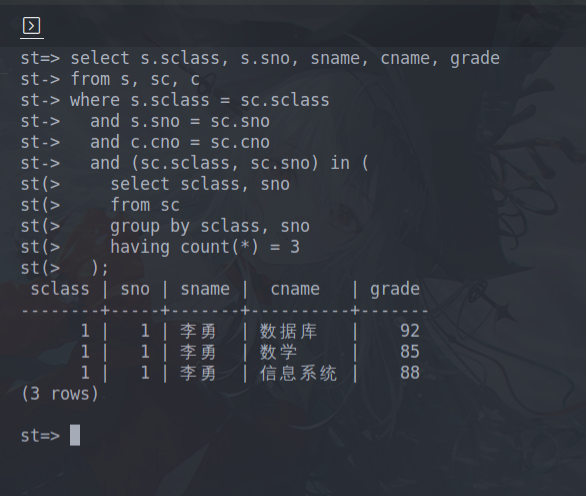
\includegraphics[width=0.8\textwidth]{23.png}
\end{center}

\end{enumerate}

\section{实验总结}

\begin{enumerate}
	\item 实验中发现建立了 ST 表之后依然找不到所创建的 ST 表,发现是被转换成了小写的 st
	\item 一开始敲入语句之后没有任何反应,发现是没有加最后的分号
	\item 学习掌握了 openGauss 数据库的安装和使用方法,并且掌握了 SQL 语句的操作
\end{enumerate}

\end{document}
